\begin{figure}[htp]
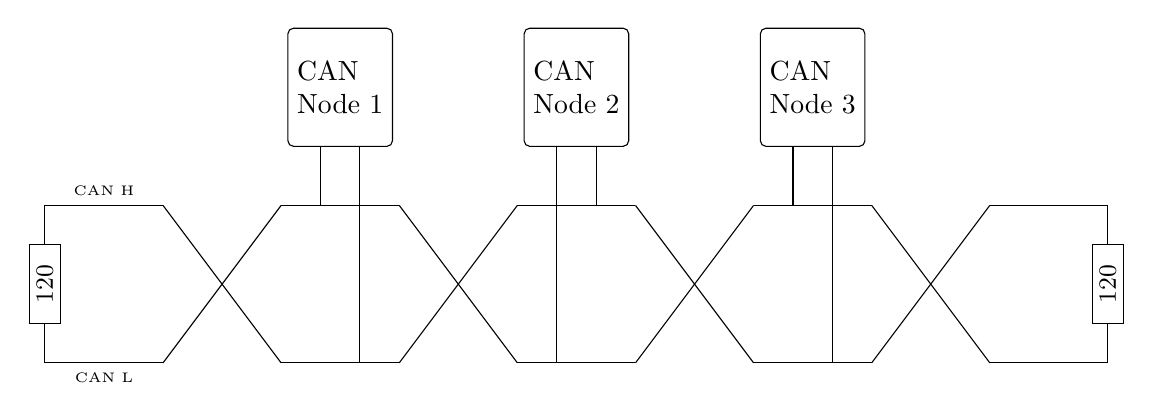
\begin{tikzpicture}
	\draw (0 cm, 0 cm) -- (1.5 cm, 0 cm) node[midway, below] {\tiny CAN L};
	\draw (0 cm, 2 cm) -- (1.5 cm, 2 cm) node[midway, above] {\tiny CAN H};
	\foreach \x in {3,6,9,12}{
		\draw (\x cm, 0 cm) -- (\x cm + 1.5 cm, 0 cm);
		\draw (\x cm, 2 cm) -- (\x cm + 1.5 cm, 2 cm);
	}
	\foreach \x in {1.5,4.5,7.5,10.5}{
		\draw (\x cm, 0 cm) -- (\x cm + 1.5 cm, 2 cm);
		\draw (\x cm, 2 cm) -- (\x cm + 1.5 cm, 0 cm);
	}
	\foreach \x in {0,13.5}{
		\draw (\x cm, 0 cm) -- (\x cm, 0.5 cm);
		\draw (\x cm - 0.2 cm, 0.5 cm) rectangle ++(0.4 cm,1 cm);
		\draw (\x cm, 2 cm) -- (\x cm, 1.5 cm);
		\node[rotate = 90] at (\x cm, 1cm) {\small120};
	}
	\node[draw, align=left, rounded corners=2pt, minimum height=1.5cm] (Node 1) at (3.75 cm,3.5 cm) {CAN \\Node 1};
	\draw (3.5 cm, 2cm) -- (3.5 cm, 2.75cm);
	\draw (4 cm, 0cm) -- (4 cm, 2.75cm);
	\node[draw, align=left, rounded corners=2pt, minimum height=1.5cm] (Node 2) at (6.75 cm,3.5 cm) {CAN \\Node 2};
	\draw (6.5 cm, 0cm) -- (6.5 cm, 2.75cm);
	\draw (7 cm, 2cm) -- (7 cm, 2.75cm);
	\node[draw, align=left, rounded corners=2pt, minimum height=1.5cm] (Node 2) at (9.75 cm,3.5 cm) {CAN \\Node 3};
	\draw (9.5 cm, 2cm) -- (9.5 cm, 2.75cm);
	\draw (10 cm, 0cm) -- (10 cm, 2.75cm);
\end{tikzpicture}
\caption{CAN Wiring}
\label{fig:can_wiring}
\end{figure}